% Options for packages loaded elsewhere
\PassOptionsToPackage{unicode}{hyperref}
\PassOptionsToPackage{hyphens}{url}
%
\documentclass[
]{article}
\usepackage{amsmath,amssymb}
\usepackage{iftex}
\ifPDFTeX
  \usepackage[T1]{fontenc}
  \usepackage[utf8]{inputenc}
  \usepackage{textcomp} % provide euro and other symbols
\else % if luatex or xetex
  \usepackage{unicode-math} % this also loads fontspec
  \defaultfontfeatures{Scale=MatchLowercase}
  \defaultfontfeatures[\rmfamily]{Ligatures=TeX,Scale=1}
\fi
\usepackage{lmodern}
\ifPDFTeX\else
  % xetex/luatex font selection
\fi
% Use upquote if available, for straight quotes in verbatim environments
\IfFileExists{upquote.sty}{\usepackage{upquote}}{}
\IfFileExists{microtype.sty}{% use microtype if available
  \usepackage[]{microtype}
  \UseMicrotypeSet[protrusion]{basicmath} % disable protrusion for tt fonts
}{}
\makeatletter
\@ifundefined{KOMAClassName}{% if non-KOMA class
  \IfFileExists{parskip.sty}{%
    \usepackage{parskip}
  }{% else
    \setlength{\parindent}{0pt}
    \setlength{\parskip}{6pt plus 2pt minus 1pt}}
}{% if KOMA class
  \KOMAoptions{parskip=half}}
\makeatother
\usepackage{xcolor}
\usepackage[margin=1in]{geometry}
\usepackage{color}
\usepackage{fancyvrb}
\newcommand{\VerbBar}{|}
\newcommand{\VERB}{\Verb[commandchars=\\\{\}]}
\DefineVerbatimEnvironment{Highlighting}{Verbatim}{commandchars=\\\{\}}
% Add ',fontsize=\small' for more characters per line
\usepackage{framed}
\definecolor{shadecolor}{RGB}{248,248,248}
\newenvironment{Shaded}{\begin{snugshade}}{\end{snugshade}}
\newcommand{\AlertTok}[1]{\textcolor[rgb]{0.94,0.16,0.16}{#1}}
\newcommand{\AnnotationTok}[1]{\textcolor[rgb]{0.56,0.35,0.01}{\textbf{\textit{#1}}}}
\newcommand{\AttributeTok}[1]{\textcolor[rgb]{0.13,0.29,0.53}{#1}}
\newcommand{\BaseNTok}[1]{\textcolor[rgb]{0.00,0.00,0.81}{#1}}
\newcommand{\BuiltInTok}[1]{#1}
\newcommand{\CharTok}[1]{\textcolor[rgb]{0.31,0.60,0.02}{#1}}
\newcommand{\CommentTok}[1]{\textcolor[rgb]{0.56,0.35,0.01}{\textit{#1}}}
\newcommand{\CommentVarTok}[1]{\textcolor[rgb]{0.56,0.35,0.01}{\textbf{\textit{#1}}}}
\newcommand{\ConstantTok}[1]{\textcolor[rgb]{0.56,0.35,0.01}{#1}}
\newcommand{\ControlFlowTok}[1]{\textcolor[rgb]{0.13,0.29,0.53}{\textbf{#1}}}
\newcommand{\DataTypeTok}[1]{\textcolor[rgb]{0.13,0.29,0.53}{#1}}
\newcommand{\DecValTok}[1]{\textcolor[rgb]{0.00,0.00,0.81}{#1}}
\newcommand{\DocumentationTok}[1]{\textcolor[rgb]{0.56,0.35,0.01}{\textbf{\textit{#1}}}}
\newcommand{\ErrorTok}[1]{\textcolor[rgb]{0.64,0.00,0.00}{\textbf{#1}}}
\newcommand{\ExtensionTok}[1]{#1}
\newcommand{\FloatTok}[1]{\textcolor[rgb]{0.00,0.00,0.81}{#1}}
\newcommand{\FunctionTok}[1]{\textcolor[rgb]{0.13,0.29,0.53}{\textbf{#1}}}
\newcommand{\ImportTok}[1]{#1}
\newcommand{\InformationTok}[1]{\textcolor[rgb]{0.56,0.35,0.01}{\textbf{\textit{#1}}}}
\newcommand{\KeywordTok}[1]{\textcolor[rgb]{0.13,0.29,0.53}{\textbf{#1}}}
\newcommand{\NormalTok}[1]{#1}
\newcommand{\OperatorTok}[1]{\textcolor[rgb]{0.81,0.36,0.00}{\textbf{#1}}}
\newcommand{\OtherTok}[1]{\textcolor[rgb]{0.56,0.35,0.01}{#1}}
\newcommand{\PreprocessorTok}[1]{\textcolor[rgb]{0.56,0.35,0.01}{\textit{#1}}}
\newcommand{\RegionMarkerTok}[1]{#1}
\newcommand{\SpecialCharTok}[1]{\textcolor[rgb]{0.81,0.36,0.00}{\textbf{#1}}}
\newcommand{\SpecialStringTok}[1]{\textcolor[rgb]{0.31,0.60,0.02}{#1}}
\newcommand{\StringTok}[1]{\textcolor[rgb]{0.31,0.60,0.02}{#1}}
\newcommand{\VariableTok}[1]{\textcolor[rgb]{0.00,0.00,0.00}{#1}}
\newcommand{\VerbatimStringTok}[1]{\textcolor[rgb]{0.31,0.60,0.02}{#1}}
\newcommand{\WarningTok}[1]{\textcolor[rgb]{0.56,0.35,0.01}{\textbf{\textit{#1}}}}
\usepackage{graphicx}
\makeatletter
\def\maxwidth{\ifdim\Gin@nat@width>\linewidth\linewidth\else\Gin@nat@width\fi}
\def\maxheight{\ifdim\Gin@nat@height>\textheight\textheight\else\Gin@nat@height\fi}
\makeatother
% Scale images if necessary, so that they will not overflow the page
% margins by default, and it is still possible to overwrite the defaults
% using explicit options in \includegraphics[width, height, ...]{}
\setkeys{Gin}{width=\maxwidth,height=\maxheight,keepaspectratio}
% Set default figure placement to htbp
\makeatletter
\def\fps@figure{htbp}
\makeatother
\setlength{\emergencystretch}{3em} % prevent overfull lines
\providecommand{\tightlist}{%
  \setlength{\itemsep}{0pt}\setlength{\parskip}{0pt}}
\setcounter{secnumdepth}{-\maxdimen} % remove section numbering
\ifLuaTeX
  \usepackage{selnolig}  % disable illegal ligatures
\fi
\IfFileExists{bookmark.sty}{\usepackage{bookmark}}{\usepackage{hyperref}}
\IfFileExists{xurl.sty}{\usepackage{xurl}}{} % add URL line breaks if available
\urlstyle{same}
\hypersetup{
  pdftitle={MA7007 - Statistical Modelling and Forecasting Case Study Report 2023-2024},
  hidelinks,
  pdfcreator={LaTeX via pandoc}}

\title{MA7007 - Statistical Modelling and Forecasting Case Study Report
2023-2024}
\author{}
\date{\vspace{-2.5em}}

\begin{document}
\maketitle

This document describes the coursework for MA7007. The coursework
involves the statistical analysis of real data sets in R and the writing
of a report to describe the results. {[}Note, the emphasis is on the
report, which means that producing just computer output it is not
enough. The output should be complimented with intelligent comments and
explanations{]}.

The coursework consists of the following:

\begin{itemize}
\item
  Each student is given two datasets.
\item
  Each student is required to find a third dataset, related to their own
  interest.
\item
  Each student is expected to analyse the first two datasets following
  the instructions given below.
\item
  For the third dataset the student is required to show their own
  initiative in analysing the data.
\item
  Each student should write a small report (less than 5000 words)
  describing how they have done the three analyses and describing their
  results. Section 2 gives instructions on writing the report.
\end{itemize}

To address the given task, we'll go through it step by step, writing R
code for each part. The task involves analyzing BMI data for Dutch boys
aged 10 to 11 years from the \texttt{dbbmi} dataset in the
\texttt{gamlss.data} package, fitting parametric distributions, and
selecting an appropriate one based on the analysis.

\hypertarget{instructions-on-how-to-analyse-the-second-data-set}{%
\subsection{Instructions on how to analyse the second data
set}\label{instructions-on-how-to-analyse-the-second-data-set}}

Cohen et al.~(2010) {[}3{]} analysed the handgrip (HG) strength in
relation to gender and age in English schoolchildren. Here each student
is required to analyse a different sample of 1000 from the original 3766
English boys. The data are stored in the packages gamlss.data under the
name grip and contain the variables grip and age. The aim here is to
create centile curves for grip given age.

\begin{Shaded}
\begin{Highlighting}[]
\CommentTok{\# Install if not already installed}
\ControlFlowTok{if}\NormalTok{ (}\SpecialCharTok{!}\FunctionTok{requireNamespace}\NormalTok{(}\StringTok{"gamlss"}\NormalTok{, }\AttributeTok{quietly =} \ConstantTok{TRUE}\NormalTok{)) }\FunctionTok{install.packages}\NormalTok{(}\StringTok{"gamlss"}\NormalTok{)}
\ControlFlowTok{if}\NormalTok{ (}\SpecialCharTok{!}\FunctionTok{requireNamespace}\NormalTok{(}\StringTok{"gamlss.data"}\NormalTok{, }\AttributeTok{quietly =} \ConstantTok{TRUE}\NormalTok{)) }\FunctionTok{install.packages}\NormalTok{(}\StringTok{"gamlss.data"}\NormalTok{)}

\CommentTok{\# Load the packages}
\FunctionTok{library}\NormalTok{(gamlss)}
\end{Highlighting}
\end{Shaded}

\begin{verbatim}
## Loading required package: splines
\end{verbatim}

\begin{verbatim}
## Loading required package: gamlss.data
\end{verbatim}

\begin{verbatim}
## 
## Attaching package: 'gamlss.data'
\end{verbatim}

\begin{verbatim}
## The following object is masked from 'package:datasets':
## 
##     sleep
\end{verbatim}

\begin{verbatim}
## Loading required package: gamlss.dist
\end{verbatim}

\begin{verbatim}
## Loading required package: nlme
\end{verbatim}

\begin{verbatim}
## Loading required package: parallel
\end{verbatim}

\begin{verbatim}
##  **********   GAMLSS Version 5.4-20  **********
\end{verbatim}

\begin{verbatim}
## For more on GAMLSS look at https://www.gamlss.com/
\end{verbatim}

\begin{verbatim}
## Type gamlssNews() to see new features/changes/bug fixes.
\end{verbatim}

\begin{Shaded}
\begin{Highlighting}[]
\FunctionTok{library}\NormalTok{(gamlss.data)}
\FunctionTok{library}\NormalTok{(MASS)}
\FunctionTok{library}\NormalTok{(gamlss)}
\FunctionTok{library}\NormalTok{(ggplot2)}
\FunctionTok{library}\NormalTok{(gamlss.ggplots)}
\end{Highlighting}
\end{Shaded}

\begin{verbatim}
## Warning: package 'gamlss.ggplots' was built under R version 4.3.3
\end{verbatim}

\begin{verbatim}
## Loading required package: gamlss.foreach
\end{verbatim}

\begin{verbatim}
## Warning: package 'gamlss.foreach' was built under R version 4.3.3
\end{verbatim}

\begin{verbatim}
## Loading required package: foreach
\end{verbatim}

\begin{verbatim}
## Loading required package: doParallel
\end{verbatim}

\begin{verbatim}
## Warning: package 'doParallel' was built under R version 4.3.3
\end{verbatim}

\begin{verbatim}
## Loading required package: iterators
\end{verbatim}

\hypertarget{a-read-the-data-file-by-typing-datagripinto-r.-note-that-the-gamlss-packages-have-to-be-downloaded-first-i.e.-librarygamlss.}{%
\subsubsection{(a) Read the data file by typing data(grip)into R. Note
that the gamlss packages have to be downloaded first
i.e.~library(gamlss).}\label{a-read-the-data-file-by-typing-datagripinto-r.-note-that-the-gamlss-packages-have-to-be-downloaded-first-i.e.-librarygamlss.}}

\hypertarget{b-in-order-to-select-your-individual-sample-a-unique-seed-number-will-be-given-to-you.-in-the-example-below-we-use-the-seed-number-243-for-demonstration.}{%
\subsubsection{(b) In order to select your individual sample a unique
seed number will be given to you. (In the example below we use the seed
number 243 for
demonstration.)}\label{b-in-order-to-select-your-individual-sample-a-unique-seed-number-will-be-given-to-you.-in-the-example-below-we-use-the-seed-number-243-for-demonstration.}}

\begin{Shaded}
\begin{Highlighting}[]
\CommentTok{\# Load the data}
\FunctionTok{data}\NormalTok{(}\StringTok{"grip"}\NormalTok{, }\AttributeTok{package =} \StringTok{"gamlss.data"}\NormalTok{)}

\FunctionTok{set.seed}\NormalTok{(}\DecValTok{243}\NormalTok{) }
\NormalTok{index }\OtherTok{\textless{}{-}} \FunctionTok{sample}\NormalTok{(}\DecValTok{3766}\NormalTok{, }\DecValTok{1000}\NormalTok{) }
\NormalTok{mydata }\OtherTok{\textless{}{-}}\NormalTok{ grip[index, ] }
\FunctionTok{dim}\NormalTok{(mydata)}
\end{Highlighting}
\end{Shaded}

\begin{verbatim}
## [1] 1000    2
\end{verbatim}

\begin{Shaded}
\begin{Highlighting}[]
\CommentTok{\# Sample 1000 observations}
\NormalTok{index }\OtherTok{\textless{}{-}} \FunctionTok{sample}\NormalTok{(}\FunctionTok{nrow}\NormalTok{(grip), }\DecValTok{1000}\NormalTok{)}
\NormalTok{grip\_sample }\OtherTok{\textless{}{-}}\NormalTok{ grip[index, ]}
\FunctionTok{dim}\NormalTok{(grip\_sample)}
\end{Highlighting}
\end{Shaded}

\begin{verbatim}
## [1] 1000    2
\end{verbatim}

\hypertarget{c-plot-grip-against-age.-note-that-there-is-no-need-to-power-transform-the-age-in-this-data-set.-explain-why.}{%
\subsubsection{(c) Plot grip against age. Note that there is no need to
power transform the age in this data set. Explain
why.}\label{c-plot-grip-against-age.-note-that-there-is-no-need-to-power-transform-the-age-in-this-data-set.-explain-why.}}

Why No Power Transformation is Necessary:

\begin{itemize}
\item
  Linearity: If the relationship between age and grip strength is linear
  or close to linear, applying a transformation to age would not yield
  any significant benefits in terms of linear regression modeling or
  interpretation.
\item
  Variability: Power transformations are also used to stabilize variance
  across the range of predictor variables. If the variance of grip
  strength is relatively constant across ages, then transforming age
  wouldn't help in stabilizing variance.
\item
  Normality of Residuals: Another reason for transformations could be to
  achieve normality of residuals in regression modeling. If the
  residuals from a model with age predicting grip strength are already
  approximately normally distributed, a transformation is unnecessary.
\item
  Simplicity: Avoiding unnecessary transformations keeps the model
  simpler and makes interpretation more straightforward. If a simple
  model without transformation provides satisfactory results, it's often
  preferred for ease of explanation and understanding.
\end{itemize}

\begin{Shaded}
\begin{Highlighting}[]
\CommentTok{\# Plot grip against age}
\FunctionTok{plot}\NormalTok{(grip}\SpecialCharTok{$}\NormalTok{age, grip}\SpecialCharTok{$}\NormalTok{grip,}
     \AttributeTok{xlab =} \StringTok{"Age"}\NormalTok{,}
     \AttributeTok{ylab =} \StringTok{"Grip Strength"}\NormalTok{,}
     \AttributeTok{main =} \StringTok{"Grip Strength vs Age"}\NormalTok{,}
     \AttributeTok{col =} \StringTok{"blue"}\NormalTok{,}
     \AttributeTok{pch =} \DecValTok{19}\NormalTok{)}

\CommentTok{\# Optional: Add a smooth line to highlight the trend}
\FunctionTok{lines}\NormalTok{(}\FunctionTok{smooth.spline}\NormalTok{(grip}\SpecialCharTok{$}\NormalTok{age, grip}\SpecialCharTok{$}\NormalTok{grip), }\AttributeTok{col =} \StringTok{"red"}\NormalTok{)}
\end{Highlighting}
\end{Shaded}

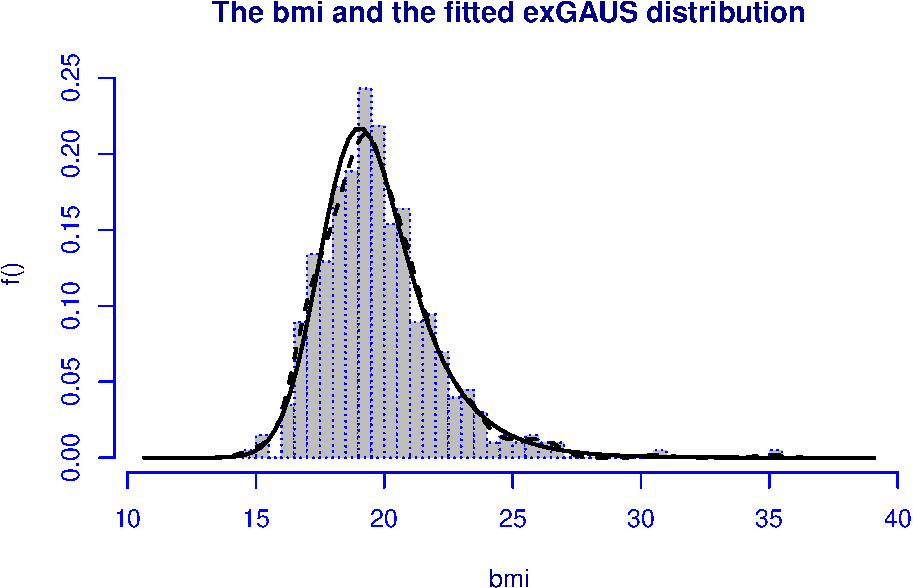
\includegraphics{Assignment-Q2_files/figure-latex/unnamed-chunk-3-1.pdf}

\begin{Shaded}
\begin{Highlighting}[]
\CommentTok{\# Plot grip against age}
\FunctionTok{plot}\NormalTok{(grip\_sample}\SpecialCharTok{$}\NormalTok{age, grip\_sample}\SpecialCharTok{$}\NormalTok{grip,}
     \AttributeTok{xlab =} \StringTok{"Age"}\NormalTok{,}
     \AttributeTok{ylab =} \StringTok{"Grip Strength"}\NormalTok{,}
     \AttributeTok{main =} \StringTok{"Grip Strength vs Age"}\NormalTok{,}
     \AttributeTok{col =} \StringTok{"blue"}\NormalTok{,}
     \AttributeTok{pch =} \DecValTok{19}\NormalTok{)}

\CommentTok{\# Optional: Add a smooth line to highlight the trend}
\FunctionTok{lines}\NormalTok{(}\FunctionTok{smooth.spline}\NormalTok{(grip\_sample}\SpecialCharTok{$}\NormalTok{age, grip\_sample}\SpecialCharTok{$}\NormalTok{grip), }\AttributeTok{col =} \StringTok{"red"}\NormalTok{)}
\end{Highlighting}
\end{Shaded}

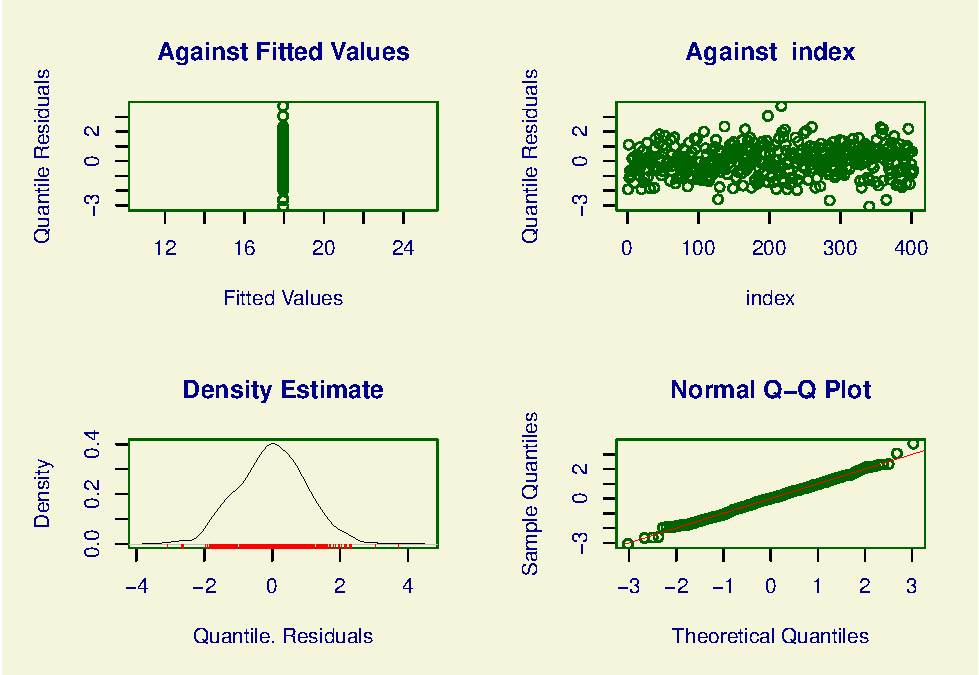
\includegraphics{Assignment-Q2_files/figure-latex/unnamed-chunk-3-2.pdf}

\hypertarget{d-use-the-lms-method-to-fit-the-data-you-can-simplify-some-of-the-steps-below-by-using-the-gamlss-package-function-lms-but-you-still-have-to-justify-the-choice-of-the-final-model.-that-is-fit-the-bccg-distribution-for-grip.}{%
\subsubsection{(d) Use the LMS method to fit the data (You can simplify
some of the steps below by using the gamlss package function lms() but
you still have to justify the choice of the final model.) That is, fit
the BCCG distribution for
grip.}\label{d-use-the-lms-method-to-fit-the-data-you-can-simplify-some-of-the-steps-below-by-using-the-gamlss-package-function-lms-but-you-still-have-to-justify-the-choice-of-the-final-model.-that-is-fit-the-bccg-distribution-for-grip.}}

gbccg \textless- gamlss(grip \textasciitilde pb(age),
sigma.fo=\textasciitilde pb(age), nu.fo=\textasciitilde pb(age),
data=da, family=BCCG)

where the smoothing for age uses the P-splines function pb(),
i.e.~pb(age), for the predictors for parameter \(\mu\), \(\sigma\) and
\(\nu\).

How many degrees of freedom were used for smoothing in the model? Use
the function edf()or edfAll().

When selecting the final model, especially after using smoothing
techniques like P-splines (pb()), it's crucial to balance fit and
complexity. Here are factors to consider in justifying your model
choice:

\begin{itemize}
\tightlist
\item
  Goodness of Fit: Use diagnostic plots and goodness-of-fit statistics
  to ensure the model adequately captures the relationship between grip
  strength and age.
\item
  Complexity vs.~Simplicity: A model with more degrees of freedom can
  capture more complex relationships but risks overfitting. Ensure the
  EDF values suggest a model complex enough to capture essential
  patterns without overfitting.
\item
  Comparison with Alternative Models: If applicable, compare your chosen
  model with alternatives using information criteria like AIC or BIC,
  which penalize model complexity.
\item
  Interpretability: Ensure the model remains interpretable. While more
  complex models might provide a marginally better fit, they should not
  do so at the expense of being understandable.
\end{itemize}

The BCCG distribution is chosen for its flexibility in modeling skewed
data, which is often encountered in physical measurements like grip
strength. By adjusting for age with P-splines, the model can flexibly
accommodate nonlinear age effects on the distribution parameters of grip
strength, making it a powerful approach for analyzing such data.

\begin{Shaded}
\begin{Highlighting}[]
\CommentTok{\# Fit the model}
\NormalTok{gbccg }\OtherTok{\textless{}{-}} \FunctionTok{gamlss}\NormalTok{(grip }\SpecialCharTok{\textasciitilde{}} \FunctionTok{pb}\NormalTok{(age),}
                \AttributeTok{sigma.fo =} \SpecialCharTok{\textasciitilde{}} \FunctionTok{pb}\NormalTok{(age),}
                \AttributeTok{nu.fo =} \SpecialCharTok{\textasciitilde{}} \FunctionTok{pb}\NormalTok{(age),}
                \AttributeTok{data =}\NormalTok{ grip\_sample,}
                \AttributeTok{family =}\NormalTok{ BCCG)}
\end{Highlighting}
\end{Shaded}

\begin{verbatim}
## GAMLSS-RS iteration 1: Global Deviance = 6281.438 
## GAMLSS-RS iteration 2: Global Deviance = 6274.721 
## GAMLSS-RS iteration 3: Global Deviance = 6274.653 
## GAMLSS-RS iteration 4: Global Deviance = 6274.65 
## GAMLSS-RS iteration 5: Global Deviance = 6274.651 
## GAMLSS-RS iteration 6: Global Deviance = 6274.652
\end{verbatim}

\begin{Shaded}
\begin{Highlighting}[]
\CommentTok{\# Extract Effective Degrees of Freedom}
\NormalTok{edf\_details }\OtherTok{\textless{}{-}} \FunctionTok{edfAll}\NormalTok{(gbccg)}

\CommentTok{\# Print the EDF for each parameter}
\FunctionTok{print}\NormalTok{(edf\_details)}
\end{Highlighting}
\end{Shaded}

\begin{verbatim}
## $mu
## $mu$`pb(age)`
## [1] 4.731575
## 
## 
## $sigma
## $sigma$`pb(age)`
## [1] 3.398777
## 
## 
## $nu
## $nu$`pb(age)`
## [1] 2.000113
\end{verbatim}

\hypertarget{e-use-the-fitted-values-from-the-lms-model-in-d-as-starting-values-for-fitting-the-bct-and-the-bcpe-distributions-to-the-data}{%
\subsubsection{(e) Use the fitted values from the LMS model in (d) as
starting values for fitting the BCT and the BCPE distributions to the
data}\label{e-use-the-fitted-values-from-the-lms-model-in-d-as-starting-values-for-fitting-the-bct-and-the-bcpe-distributions-to-the-data}}

e.g.~\texttt{gbct\ \textless{}-\ gamlss(grip\textasciitilde{}pb(age),\ sigma.fo\ =\ \textasciitilde{}pb(age),\ nu.fo\ =\ \textasciitilde{}pb(age),\ tau.fo\ =\ \textasciitilde{}pb(age),\ data=da,\ family=BCT,\ start.from=gbccg)}

What are the effective degrees of freedom fitted for the parameters? Try
to interpret the effective degrees of freedom.

Interpreting the Effective Degrees of Freedom:

\begin{itemize}
\item
  EDF Near 1: If the effective degrees of freedom for a parameter is
  close to 1, it suggests that the model is applying very little
  smoothing to that parameter. This can imply a linear relationship
  between the parameter and the predictors.
\item
  EDF Greater Than 1: An EDF significantly greater than 1 indicates more
  complex relationships are being modeled, with the splines applying
  more smoothing. This is often necessary when the relationship between
  the response and predictors is nonlinear or when there's a varying
  effect of predictors across the range of the data.
\item
  High EDF: Very high EDF values may signal overfitting, where the model
  is too closely fitting the idiosyncrasies of the sample data rather
  than capturing the underlying population trends.
\end{itemize}

The mu, sigma, nu, and tau parameters represent different aspects of the
distribution being modeled:

\begin{itemize}
\tightlist
\item
  mu (\(\mu\)): The location parameter (central tendency).
\item
  sigma (\(\sigma\)): The scale parameter (dispersion or variability).
\item
  nu (\(\nu\)) and
\item
  tau (\(\tau\)): Parameters that control the shape of the distribution,
  including skewness and kurtosis.
\end{itemize}

Choosing between the BCT and BCPE models, and interpreting their
parameters' EDFs, depends on the fit quality, predictive performance,
and the complexity trade-off. This process is crucial for understanding
how age influences grip strength across its distribution and ensuring
the model's generalizability.

\begin{Shaded}
\begin{Highlighting}[]
\CommentTok{\# Fit the BCT model using gbccg as starting values}
\NormalTok{gbct }\OtherTok{\textless{}{-}} \FunctionTok{gamlss}\NormalTok{(grip }\SpecialCharTok{\textasciitilde{}} \FunctionTok{pb}\NormalTok{(age),}
               \AttributeTok{sigma.fo =} \SpecialCharTok{\textasciitilde{}} \FunctionTok{pb}\NormalTok{(age),}
               \AttributeTok{nu.fo =} \SpecialCharTok{\textasciitilde{}} \FunctionTok{pb}\NormalTok{(age),}
               \AttributeTok{tau.fo =} \SpecialCharTok{\textasciitilde{}} \FunctionTok{pb}\NormalTok{(age),}
               \AttributeTok{data =}\NormalTok{ grip\_sample,}
               \AttributeTok{family =}\NormalTok{ BCT,}
               \AttributeTok{start.from =}\NormalTok{ gbccg)}
\end{Highlighting}
\end{Shaded}

\begin{verbatim}
## GAMLSS-RS iteration 1: Global Deviance = 6250.993 
## GAMLSS-RS iteration 2: Global Deviance = 6249.203 
## GAMLSS-RS iteration 3: Global Deviance = 6248.849 
## GAMLSS-RS iteration 4: Global Deviance = 6248.755 
## GAMLSS-RS iteration 5: Global Deviance = 6248.726 
## GAMLSS-RS iteration 6: Global Deviance = 6248.717 
## GAMLSS-RS iteration 7: Global Deviance = 6248.715 
## GAMLSS-RS iteration 8: Global Deviance = 6248.714
\end{verbatim}

\begin{Shaded}
\begin{Highlighting}[]
\CommentTok{\# Fit the BCPE model using gbccg as starting values}
\NormalTok{gbcpe }\OtherTok{\textless{}{-}} \FunctionTok{gamlss}\NormalTok{(grip }\SpecialCharTok{\textasciitilde{}} \FunctionTok{pb}\NormalTok{(age),}
                \AttributeTok{sigma.fo =} \SpecialCharTok{\textasciitilde{}} \FunctionTok{pb}\NormalTok{(age),}
                \AttributeTok{nu.fo =} \SpecialCharTok{\textasciitilde{}} \FunctionTok{pb}\NormalTok{(age),}
                \AttributeTok{tau.fo =} \SpecialCharTok{\textasciitilde{}} \FunctionTok{pb}\NormalTok{(age),}
                \AttributeTok{data =}\NormalTok{ grip\_sample,}
                \AttributeTok{family =}\NormalTok{ BCPE,}
                \AttributeTok{start.from =}\NormalTok{ gbccg)}
\end{Highlighting}
\end{Shaded}

\begin{verbatim}
## GAMLSS-RS iteration 1: Global Deviance = 6245.244 
## GAMLSS-RS iteration 2: Global Deviance = 6245.354 
## GAMLSS-RS iteration 3: Global Deviance = 6245.484 
## GAMLSS-RS iteration 4: Global Deviance = 6245.505 
## GAMLSS-RS iteration 5: Global Deviance = 6245.508 
## GAMLSS-RS iteration 6: Global Deviance = 6245.507
\end{verbatim}

\begin{Shaded}
\begin{Highlighting}[]
\CommentTok{\# The EDF indicates the complexity of the model related to each parameter.}

\CommentTok{\# Extract EDF for BCT model}
\NormalTok{edf\_bct }\OtherTok{\textless{}{-}} \FunctionTok{edfAll}\NormalTok{(gbct)}

\CommentTok{\# Extract EDF for BCPE model}
\NormalTok{edf\_bcpe }\OtherTok{\textless{}{-}} \FunctionTok{edfAll}\NormalTok{(gbcpe)}

\CommentTok{\# Print the EDF for each model}
\FunctionTok{print}\NormalTok{(edf\_bct)}
\end{Highlighting}
\end{Shaded}

\begin{verbatim}
## $mu
## $mu$`pb(age)`
## [1] 4.756824
## 
## 
## $sigma
## $sigma$`pb(age)`
## [1] 3.467468
## 
## 
## $nu
## $nu$`pb(age)`
## [1] 2.000118
## 
## 
## $tau
## $tau$`pb(age)`
## [1] 2.000039
\end{verbatim}

\begin{Shaded}
\begin{Highlighting}[]
\FunctionTok{print}\NormalTok{(edf\_bcpe)}
\end{Highlighting}
\end{Shaded}

\begin{verbatim}
## $mu
## $mu$`pb(age)`
## [1] 4.80843
## 
## 
## $sigma
## $sigma$`pb(age)`
## [1] 3.14181
## 
## 
## $nu
## $nu$`pb(age)`
## [1] 2.00009
## 
## 
## $tau
## $tau$`pb(age)`
## [1] 2.000348
\end{verbatim}

\hypertarget{f-use-the-generalised-akaike-information-criterion-gaic-to-compare-the-three-models.}{%
\subsubsection{(f) Use the generalised Akaike information criterion,
GAIC, to compare the three
models.}\label{f-use-the-generalised-akaike-information-criterion-gaic-to-compare-the-three-models.}}

The GAIC is a variant of the Akaike Information Criterion (AIC) that
allows for a more flexible penalization of model complexity and is
particularly useful in comparing models fitted with the same dataset but
different distributions or complexities.

Interpreting GAIC

When comparing models with GAIC, the model with the lowest GAIC value is
generally considered the best among the set, as it strikes the most
favorable balance between model fit and complexity. The GAIC penalizes
models more heavily for additional parameters than the traditional AIC
does, making it particularly useful for models that might overfit the
data with too many parameters or excessive flexibility.

\begin{itemize}
\item
  Lower GAIC: Indicates a model that has a better trade-off between
  goodness-of-fit and complexity, suggesting it might generalize better
  to new data.
\item
  Comparing Values: The absolute value of the GAIC is not interpretable
  on its own; it's the relative differences between the GAIC scores of
  the models that inform model selection. A difference of more than a
  few points is generally considered meaningful.
\end{itemize}

By evaluating the GAIC values for your three models, you can make an
informed decision about which model provides the best fit to your data
without unnecessarily increasing model complexity. This is particularly
useful in your case, where you're fitting different distributions and
considering different forms of the response variable's relationship with
predictors.

\begin{Shaded}
\begin{Highlighting}[]
\CommentTok{\# Calculate GAIC for each model}
\NormalTok{gaic\_bccg }\OtherTok{\textless{}{-}} \FunctionTok{GAIC}\NormalTok{(gbccg)}
\NormalTok{gaic\_gbct }\OtherTok{\textless{}{-}} \FunctionTok{GAIC}\NormalTok{(gbct)}
\NormalTok{gaic\_gbcpe }\OtherTok{\textless{}{-}} \FunctionTok{GAIC}\NormalTok{(gbcpe)}

\CommentTok{\# Print the GAIC values}
\FunctionTok{print}\NormalTok{(}\FunctionTok{paste}\NormalTok{(}\StringTok{"GAIC for BCCG:"}\NormalTok{, gaic\_bccg))}
\end{Highlighting}
\end{Shaded}

\begin{verbatim}
## [1] "GAIC for BCCG: 6294.91261769977"
\end{verbatim}

\begin{Shaded}
\begin{Highlighting}[]
\FunctionTok{print}\NormalTok{(}\FunctionTok{paste}\NormalTok{(}\StringTok{"GAIC for BCT:"}\NormalTok{, gaic\_gbct))}
\end{Highlighting}
\end{Shaded}

\begin{verbatim}
## [1] "GAIC for BCT: 6273.16293567327"
\end{verbatim}

\begin{Shaded}
\begin{Highlighting}[]
\FunctionTok{print}\NormalTok{(}\FunctionTok{paste}\NormalTok{(}\StringTok{"GAIC for BCPE:"}\NormalTok{, gaic\_gbcpe))}
\end{Highlighting}
\end{Shaded}

\begin{verbatim}
## [1] "GAIC for BCPE: 6269.4088588138"
\end{verbatim}

\hypertarget{g-plot-the-fitted-parameters-for-the-fitted-models-in-d-and-e-using-for-example}{%
\subsubsection{(g) Plot the fitted parameters for the fitted models in
(d) and (e) using for
example}\label{g-plot-the-fitted-parameters-for-the-fitted-models-in-d-and-e-using-for-example}}

\texttt{fitted.plot(gbccg,\ gbct,\ x=da\$age)} where gbccg and gbct are
the BCCG and BCT models respectively.

\begin{Shaded}
\begin{Highlighting}[]
\CommentTok{\# Assuming \textquotesingle{}grip\_sample\textquotesingle{} is your dataset and \textquotesingle{}gbccg\textquotesingle{} and \textquotesingle{}gbct\textquotesingle{} are fitted models}
\FunctionTok{fittedPlot}\NormalTok{(gbccg, gbct, }\AttributeTok{x=}\NormalTok{grip\_sample}\SpecialCharTok{$}\NormalTok{age)}
\end{Highlighting}
\end{Shaded}

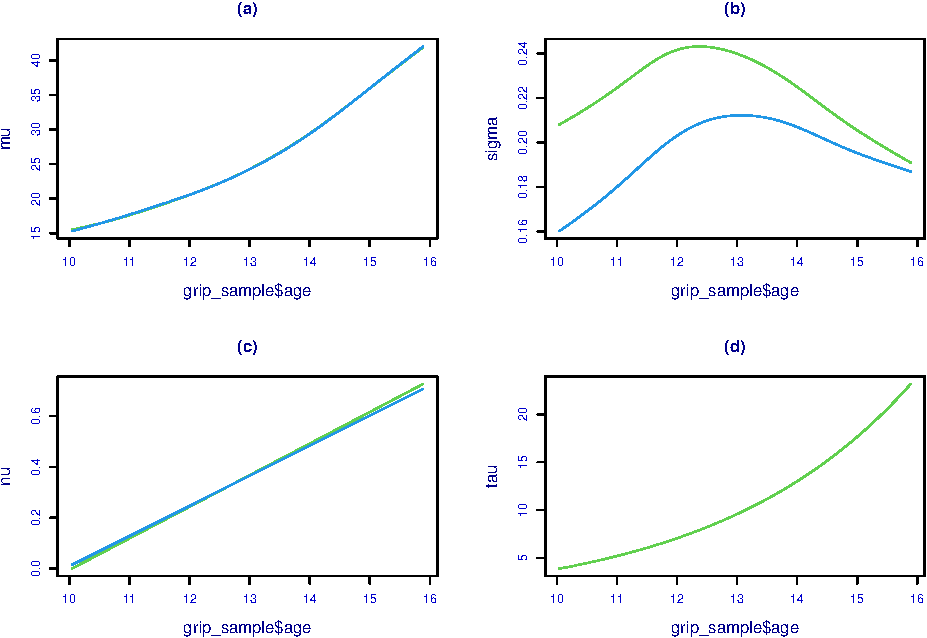
\includegraphics{Assignment-Q2_files/figure-latex/unnamed-chunk-7-1.pdf}

\begin{Shaded}
\begin{Highlighting}[]
\CommentTok{\# Calculate fitted values or centiles for each model across a range of ages}
\NormalTok{age\_seq }\OtherTok{\textless{}{-}} \FunctionTok{seq}\NormalTok{(}\FunctionTok{min}\NormalTok{(grip\_sample}\SpecialCharTok{$}\NormalTok{age), }\FunctionTok{max}\NormalTok{(grip\_sample}\SpecialCharTok{$}\NormalTok{age), }\AttributeTok{length.out =} \DecValTok{100}\NormalTok{)}

\CommentTok{\# For BCCG Model}
\NormalTok{fitted\_bccg }\OtherTok{\textless{}{-}} \FunctionTok{predict}\NormalTok{(gbccg, }\AttributeTok{newdata=}\FunctionTok{data.frame}\NormalTok{(}\AttributeTok{age=}\NormalTok{age\_seq), }\AttributeTok{type=}\StringTok{"response"}\NormalTok{)}
\end{Highlighting}
\end{Shaded}

\begin{verbatim}
## new prediction
\end{verbatim}

\begin{Shaded}
\begin{Highlighting}[]
\CommentTok{\# For BCT Model}
\NormalTok{fitted\_gbct }\OtherTok{\textless{}{-}} \FunctionTok{predict}\NormalTok{(gbct, }\AttributeTok{newdata=}\FunctionTok{data.frame}\NormalTok{(}\AttributeTok{age=}\NormalTok{age\_seq), }\AttributeTok{type=}\StringTok{"response"}\NormalTok{)}
\end{Highlighting}
\end{Shaded}

\begin{verbatim}
## new prediction
\end{verbatim}

\begin{Shaded}
\begin{Highlighting}[]
\CommentTok{\# Plotting}
\FunctionTok{plot}\NormalTok{(age\_seq, fitted\_bccg, }\AttributeTok{type=}\StringTok{\textquotesingle{}l\textquotesingle{}}\NormalTok{, }\AttributeTok{col=}\StringTok{\textquotesingle{}blue\textquotesingle{}}\NormalTok{, }\AttributeTok{ylim=}\FunctionTok{range}\NormalTok{(}\FunctionTok{c}\NormalTok{(fitted\_bccg, fitted\_gbct)),}
     \AttributeTok{xlab=}\StringTok{\textquotesingle{}Age\textquotesingle{}}\NormalTok{, }\AttributeTok{ylab=}\StringTok{\textquotesingle{}Fitted Grip Strength\textquotesingle{}}\NormalTok{, }\AttributeTok{main=}\StringTok{\textquotesingle{}Fitted Models Comparison\textquotesingle{}}\NormalTok{)}
\FunctionTok{lines}\NormalTok{(age\_seq, fitted\_gbct, }\AttributeTok{col=}\StringTok{\textquotesingle{}red\textquotesingle{}}\NormalTok{)}

\CommentTok{\# Adding a legend}
\FunctionTok{legend}\NormalTok{(}\StringTok{"topright"}\NormalTok{, }\AttributeTok{legend=}\FunctionTok{c}\NormalTok{(}\StringTok{"BCCG"}\NormalTok{, }\StringTok{"BCT"}\NormalTok{), }\AttributeTok{col=}\FunctionTok{c}\NormalTok{(}\StringTok{"blue"}\NormalTok{, }\StringTok{"red"}\NormalTok{), }\AttributeTok{lty=}\DecValTok{1}\NormalTok{, }\AttributeTok{cex=}\FloatTok{0.8}\NormalTok{)}
\end{Highlighting}
\end{Shaded}

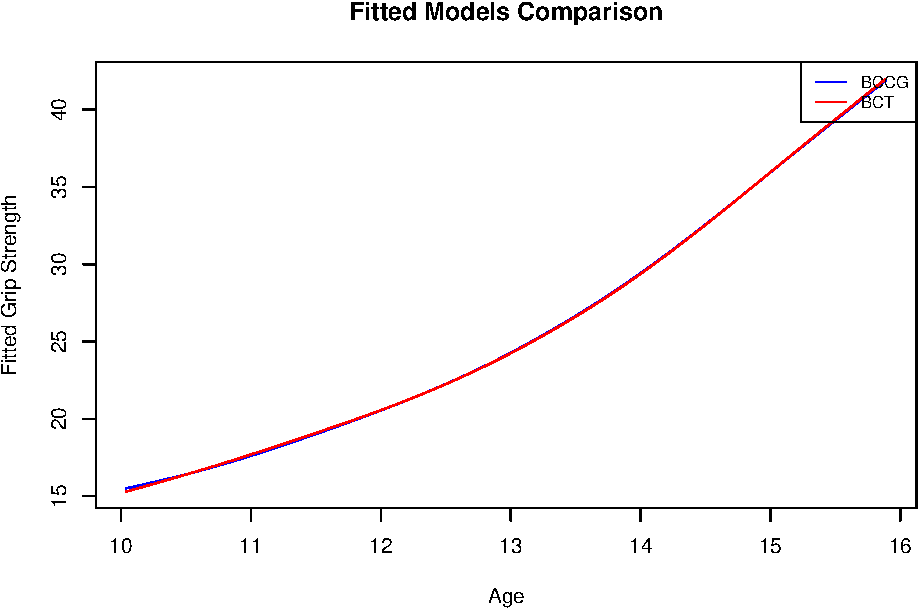
\includegraphics{Assignment-Q2_files/figure-latex/unnamed-chunk-7-2.pdf}

\hypertarget{h-obtain-a-centile-plot-for-the-fitted-models-in-d-and-e-using-centiles-orcentiles.split-and-compare-them.}{%
\subsubsection{(h) Obtain a centile plot for the fitted models in (d)
and (e) using centiles() orcentiles.split() and compare
them.}\label{h-obtain-a-centile-plot-for-the-fitted-models-in-d-and-e-using-centiles-orcentiles.split-and-compare-them.}}

Interpreting the Comparison:

\begin{itemize}
\item
  Overlap and Divergence: Overlapping lines suggest agreement between
  models in estimating grip strength across age centiles. Divergence
  indicates differences in how models estimate grip strength at various
  ages, potentially due to differences in distributional assumptions or
  how well each model captures the variability in the data.
\item
  Model Fit and Data Representation: This visual comparison can help
  assess which model might provide a better fit or more accurately
  represent the underlying trends and variations in your data. For
  example, if one model's centiles follow the data more closely or seem
  to capture the trend without overfitting, it might be preferable.
\end{itemize}

By comparing these centile plots, you get a visual representation of how
each model performs across the range of ages, which can inform your
decision on the best model for your analysis based on how well they fit
the centiles to the observed data.

\begin{Shaded}
\begin{Highlighting}[]
\CommentTok{\#centilesTwo(gbccg, grid.x1 = age, grid.x2 = grip, )}
\FunctionTok{centiles}\NormalTok{(gbccg, }\AttributeTok{xvar=}\NormalTok{grip\_sample}\SpecialCharTok{$}\NormalTok{age, }\AttributeTok{cent=}\FunctionTok{c}\NormalTok{(}\FloatTok{0.1}\NormalTok{, }\FloatTok{0.4}\NormalTok{, }\DecValTok{2}\NormalTok{,}\DecValTok{10}\NormalTok{,}\DecValTok{25}\NormalTok{,}\DecValTok{50}\NormalTok{,}\DecValTok{75}\NormalTok{,}\DecValTok{90}\NormalTok{,}\DecValTok{98}\NormalTok{,}\FloatTok{99.6}\NormalTok{, }\FloatTok{99.9}\NormalTok{), }\AttributeTok{ylab=}\StringTok{"grip"}\NormalTok{, }\AttributeTok{xlab=}\StringTok{"age"}\NormalTok{, }\AttributeTok{legend=}\ConstantTok{FALSE}\NormalTok{)}
\end{Highlighting}
\end{Shaded}

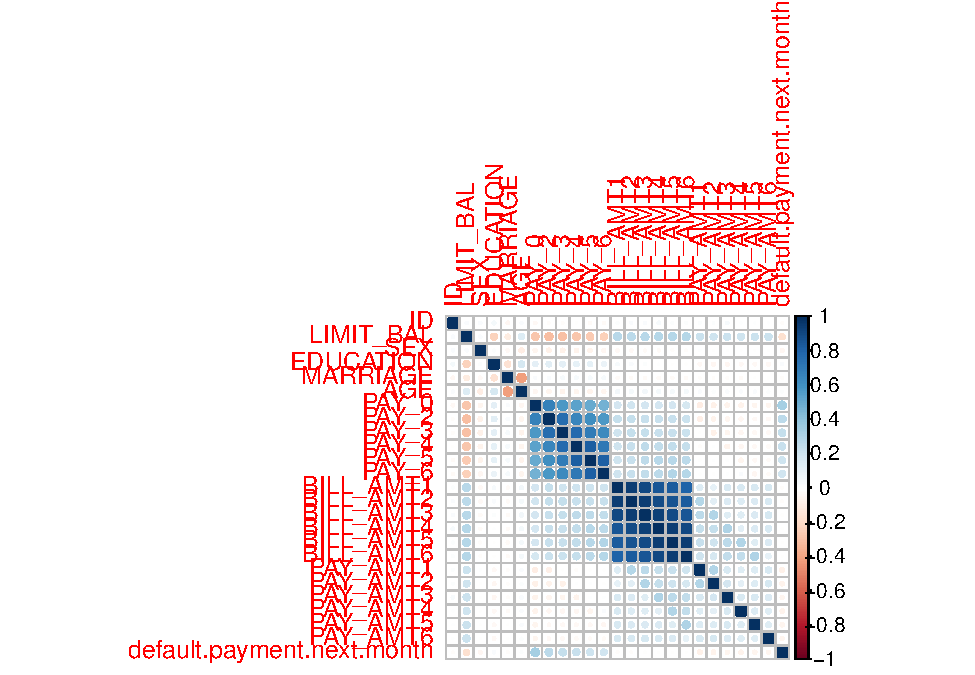
\includegraphics{Assignment-Q2_files/figure-latex/unnamed-chunk-8-1.pdf}

\begin{verbatim}
## % of cases below  0.1 centile is  0.3 
## % of cases below  0.4 centile is  0.5 
## % of cases below  2 centile is  2.5 
## % of cases below  10 centile is  9.6 
## % of cases below  25 centile is  23.7 
## % of cases below  50 centile is  49.7 
## % of cases below  75 centile is  77.6 
## % of cases below  90 centile is  90.9 
## % of cases below  98 centile is  97.8 
## % of cases below  99.6 centile is  99.2 
## % of cases below  99.9 centile is  99.5
\end{verbatim}

\begin{Shaded}
\begin{Highlighting}[]
\CommentTok{\# Plot centiles for BCCG model}
\FunctionTok{plot}\NormalTok{(grip\_sample}\SpecialCharTok{$}\NormalTok{age, grip\_sample}\SpecialCharTok{$}\NormalTok{grip, }\AttributeTok{col=}\StringTok{"gray90"}\NormalTok{, }\AttributeTok{main=}\StringTok{"Centile Comparison"}\NormalTok{, }\AttributeTok{xlab=}\StringTok{"Age"}\NormalTok{, }\AttributeTok{ylab=}\StringTok{"Grip Strength"}\NormalTok{)}
\end{Highlighting}
\end{Shaded}

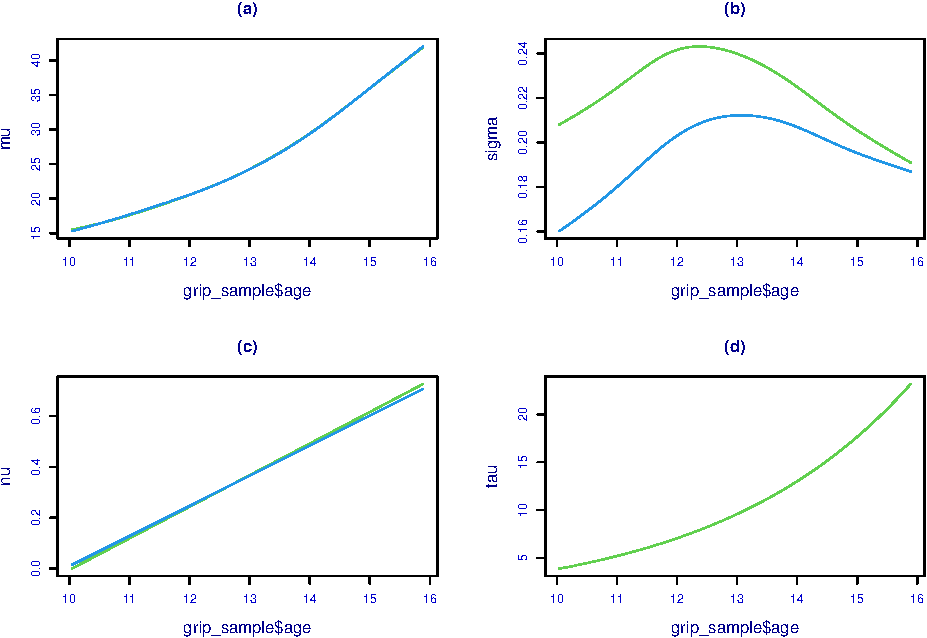
\includegraphics{Assignment-Q2_files/figure-latex/unnamed-chunk-9-1.pdf}

\begin{Shaded}
\begin{Highlighting}[]
\FunctionTok{centiles}\NormalTok{(gbccg, }\AttributeTok{xvar =}\NormalTok{ grip\_sample}\SpecialCharTok{$}\NormalTok{age, }\AttributeTok{col =} \StringTok{"blue"}\NormalTok{, }\AttributeTok{lty =} \DecValTok{1}\NormalTok{)}
\end{Highlighting}
\end{Shaded}

\begin{verbatim}
## % of cases below  0.4 centile is  0.5 
## % of cases below  2 centile is  2.5 
## % of cases below  10 centile is  9.6 
## % of cases below  25 centile is  23.7 
## % of cases below  50 centile is  49.7 
## % of cases below  75 centile is  77.6 
## % of cases below  90 centile is  90.9 
## % of cases below  98 centile is  97.8 
## % of cases below  99.6 centile is  99.2
\end{verbatim}

\begin{Shaded}
\begin{Highlighting}[]
\FunctionTok{legend}\NormalTok{(}\StringTok{"topright"}\NormalTok{, }\AttributeTok{legend=}\FunctionTok{c}\NormalTok{(}\StringTok{"BCCG"}\NormalTok{), }\AttributeTok{col=}\FunctionTok{c}\NormalTok{(}\StringTok{"blue"}\NormalTok{), }\AttributeTok{lty=}\DecValTok{1}\NormalTok{, }\AttributeTok{cex=}\FloatTok{0.8}\NormalTok{)}
\end{Highlighting}
\end{Shaded}

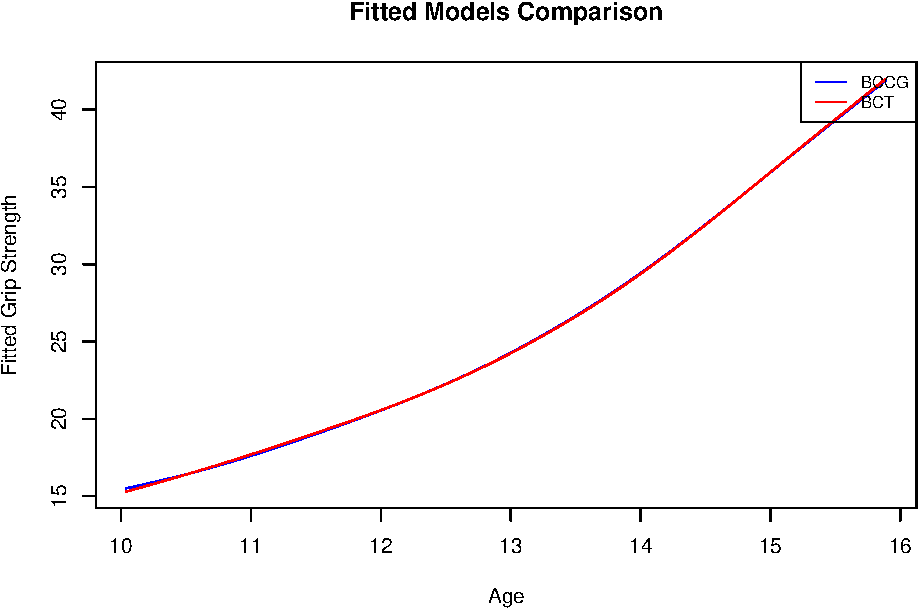
\includegraphics{Assignment-Q2_files/figure-latex/unnamed-chunk-9-2.pdf}

\begin{Shaded}
\begin{Highlighting}[]
\CommentTok{\# Add centiles for BCT model to the existing plot}
\FunctionTok{centiles}\NormalTok{(gbct, }\AttributeTok{xvar =}\NormalTok{ grip\_sample}\SpecialCharTok{$}\NormalTok{age, }\AttributeTok{col =} \StringTok{"red"}\NormalTok{, }\AttributeTok{lty =} \DecValTok{2}\NormalTok{)}
\end{Highlighting}
\end{Shaded}

\begin{verbatim}
## % of cases below  0.4 centile is  0.3 
## % of cases below  2 centile is  2.2 
## % of cases below  10 centile is  10.4 
## % of cases below  25 centile is  25.6 
## % of cases below  50 centile is  49.6 
## % of cases below  75 centile is  75.6 
## % of cases below  90 centile is  90 
## % of cases below  98 centile is  98.1 
## % of cases below  99.6 centile is  99.6
\end{verbatim}

\begin{Shaded}
\begin{Highlighting}[]
\CommentTok{\# Update the legend to include BCT}
\FunctionTok{legend}\NormalTok{(}\StringTok{"topright"}\NormalTok{, }\AttributeTok{legend=}\FunctionTok{c}\NormalTok{(}\StringTok{"BCCG"}\NormalTok{, }\StringTok{"BCT"}\NormalTok{), }\AttributeTok{col=}\FunctionTok{c}\NormalTok{(}\StringTok{"blue"}\NormalTok{, }\StringTok{"red"}\NormalTok{), }\AttributeTok{lty=}\DecValTok{1}\SpecialCharTok{:}\DecValTok{2}\NormalTok{, }\AttributeTok{cex=}\FloatTok{0.8}\NormalTok{)}
\end{Highlighting}
\end{Shaded}

\includegraphics{Assignment-Q2_files/figure-latex/unnamed-chunk-9-3.pdf}

\hypertarget{i-investigate-the-residuals-from-the-fitted-models-in-d-and-e}{%
\subsubsection{(i) Investigate the residuals from the fitted models in
(d) and
(e)}\label{i-investigate-the-residuals-from-the-fitted-models-in-d-and-e}}

using e.g.~plot(), wp() (worm plot) and Q.stats()(Q-statistics).

\hypertarget{interpreting-diagnostic-plots-and-statistics}{%
\paragraph{Interpreting Diagnostic Plots and
Statistics:}\label{interpreting-diagnostic-plots-and-statistics}}

\begin{itemize}
\item
  Residual Plots: You're looking for patterns or systematic deviations
  from zero. Ideally, residuals should be randomly distributed around
  zero without clear patterns.
\item
  Worm Plots (WP): These plots should ideally resemble a straight line.
  Curvature or deviations from the line indicate potential issues with
  the model's fit to the data, such as non-normality or
  heteroscedasticity.
\item
  Q-Statistics (Q.stats()): This provides a summary of the quantiles of
  the residuals compared to the expected distribution. Significant
  deviations can indicate that the model's assumptions about the
  distribution of residuals may not hold.
\end{itemize}

When using these diagnostic tools, it's important to consider them
collectively rather than relying on a single method. Each tool can
highlight different aspects of the model fit and potential areas for
improvement.

\begin{Shaded}
\begin{Highlighting}[]
\CommentTok{\# For BCCG Model}
\FunctionTok{plot}\NormalTok{(}\FunctionTok{residuals}\NormalTok{(gbccg), }\AttributeTok{main=}\StringTok{"Residuals for BCCG Model"}\NormalTok{)}
\end{Highlighting}
\end{Shaded}

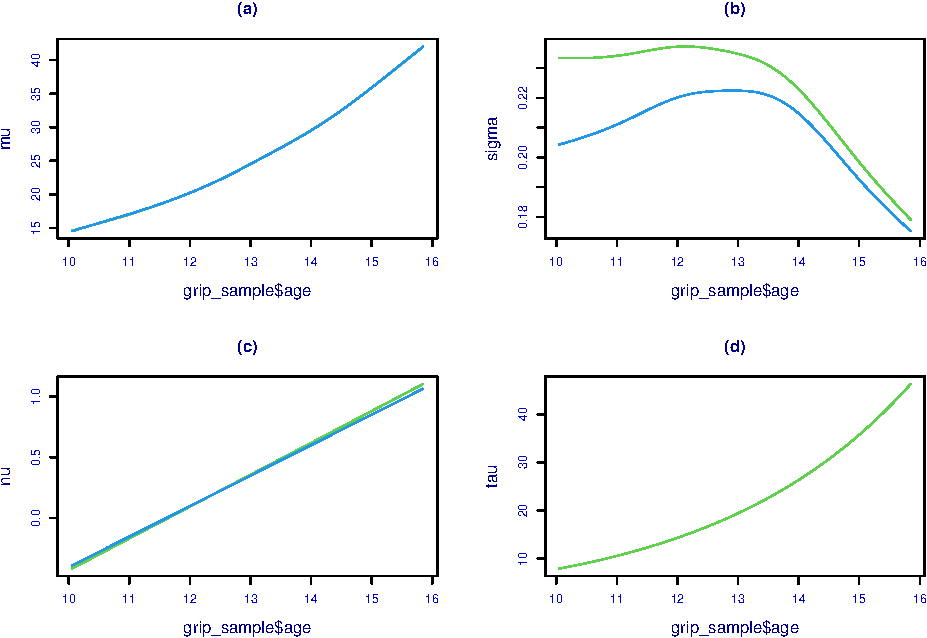
\includegraphics{Assignment-Q2_files/figure-latex/unnamed-chunk-10-1.pdf}

\begin{Shaded}
\begin{Highlighting}[]
\CommentTok{\# For BCT Model}
\FunctionTok{plot}\NormalTok{(}\FunctionTok{residuals}\NormalTok{(gbct), }\AttributeTok{main=}\StringTok{"Residuals for BCT Model"}\NormalTok{)}
\end{Highlighting}
\end{Shaded}

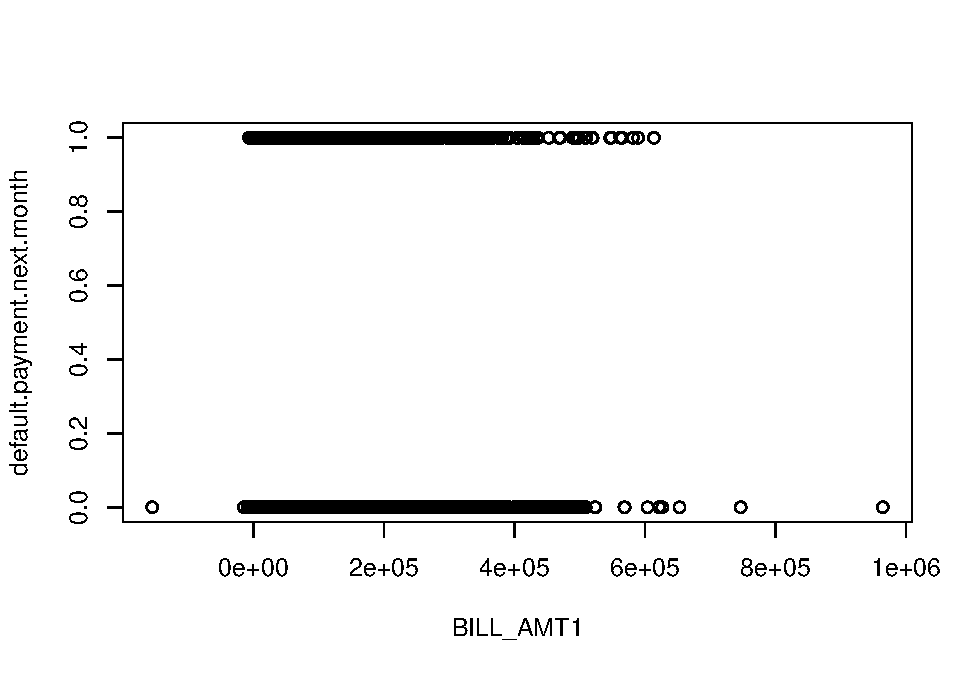
\includegraphics{Assignment-Q2_files/figure-latex/unnamed-chunk-10-2.pdf}

\begin{Shaded}
\begin{Highlighting}[]
\CommentTok{\# Assuming the \textquotesingle{}gamlss\textquotesingle{} package is loaded}

\CommentTok{\# For BCCG Model}
\FunctionTok{wp}\NormalTok{(gbccg, }\AttributeTok{main=}\StringTok{"Worm Plot for BCCG Model"}\NormalTok{)}
\end{Highlighting}
\end{Shaded}

\begin{verbatim}
## Warning in wp(gbccg, main = "Worm Plot for BCCG Model"): Some points are missed out 
## increase the y limits using ylim.all
\end{verbatim}

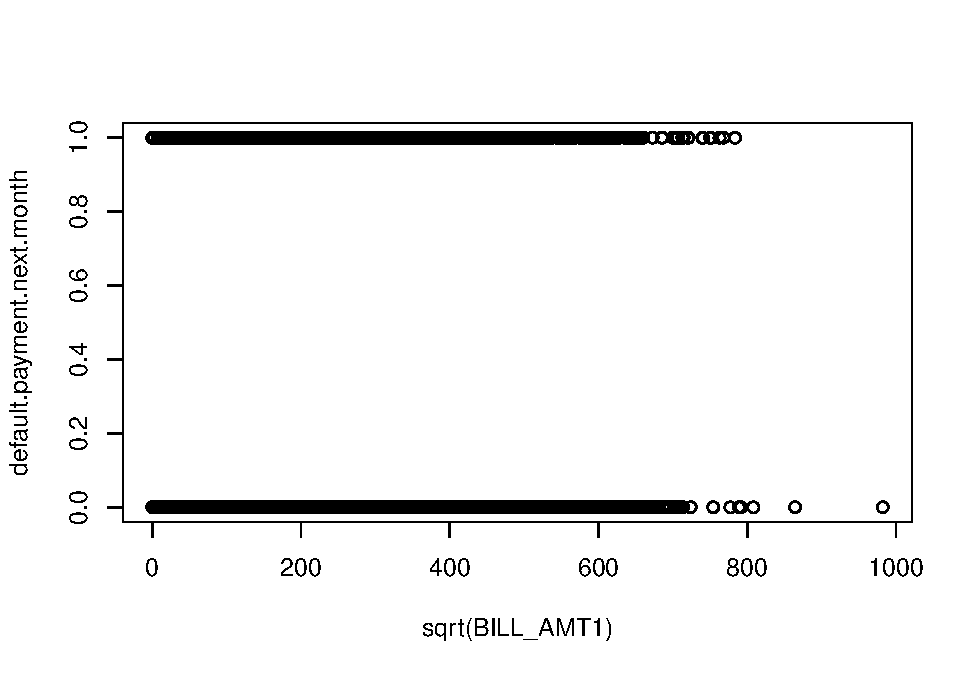
\includegraphics{Assignment-Q2_files/figure-latex/unnamed-chunk-10-3.pdf}

\begin{Shaded}
\begin{Highlighting}[]
\CommentTok{\# For BCT Model}
\FunctionTok{wp}\NormalTok{(gbct, }\AttributeTok{main=}\StringTok{"Worm Plot for BCT Model"}\NormalTok{)}
\end{Highlighting}
\end{Shaded}

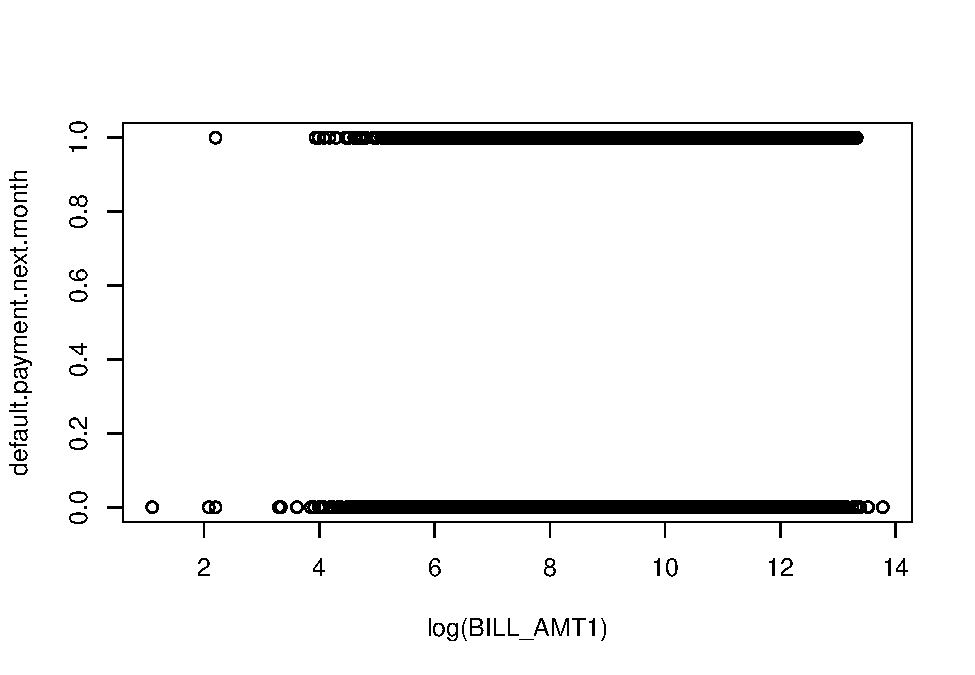
\includegraphics{Assignment-Q2_files/figure-latex/unnamed-chunk-10-4.pdf}

\begin{Shaded}
\begin{Highlighting}[]
\CommentTok{\# For BCCG Model}
\NormalTok{qstats\_bccg }\OtherTok{\textless{}{-}} \FunctionTok{Q.stats}\NormalTok{(gbccg)}
\end{Highlighting}
\end{Shaded}

\begin{verbatim}
## Warning in Q.stats(gbccg): The xvar has been replace by an index 1:n 
## 
\end{verbatim}

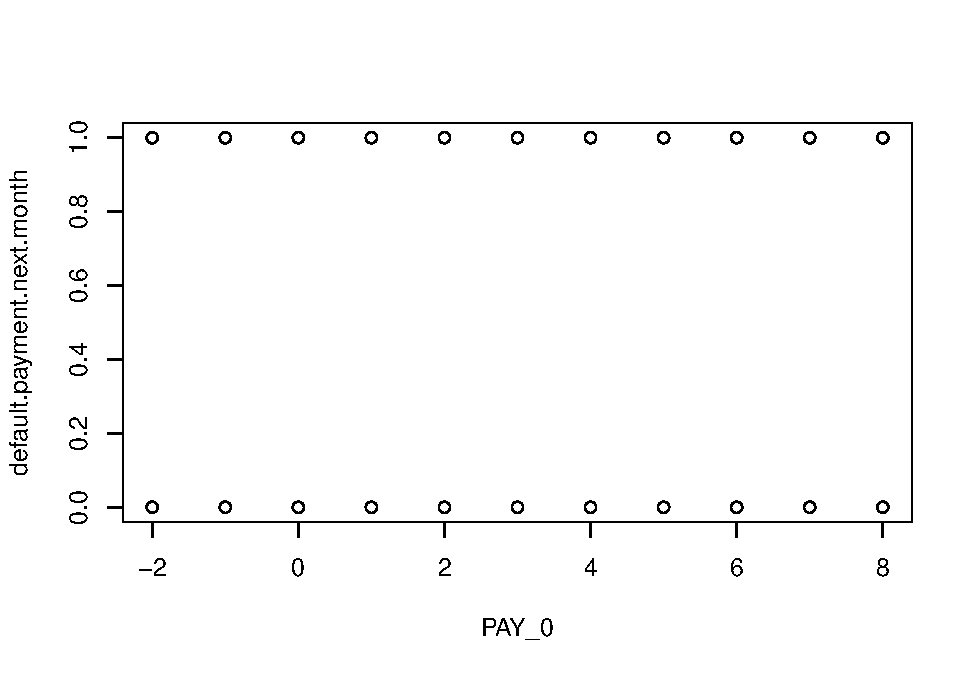
\includegraphics{Assignment-Q2_files/figure-latex/unnamed-chunk-10-5.pdf}

\begin{Shaded}
\begin{Highlighting}[]
\FunctionTok{print}\NormalTok{(qstats\_bccg)}
\end{Highlighting}
\end{Shaded}

\begin{verbatim}
##                           Z1           Z2           Z3           Z4
##    0.5 to  100.5   0.2853203 -0.539279221 -0.901130048 -0.062506720
##  100.5 to  200.5   0.7490694  2.543402307  0.914966311  0.666350041
##  200.5 to  300.5   0.1167846 -0.648368504  3.049115344  3.497164185
##  300.5 to  400.5  -0.4343136 -2.284569286 -1.026868574  0.823841198
##  400.5 to  500.5  -0.2198399 -2.763364472  1.610106996  1.526017474
##  500.5 to  600.5   0.4851420 -0.294830372  1.132835910  0.506159292
##  600.5 to  700.5   1.3256751 -0.346307455  1.029748206  1.501453854
##  700.5 to  800.5  -1.8050445  1.559110121 -2.247880791  1.608541892
##  800.5 to  900.5   0.9645853  1.125300951 -1.942720187  2.359490449
##  900.5 to 1000.5  -1.4746916  0.336865137  0.559320338  1.383083131
## TOTAL Q stats      9.2492125 24.052997641 26.076874281 28.263612501
## df for Q stats     5.2684253  7.800611395  7.999887173 10.000000000
## p-val for Q stats  0.1142045  0.001964394  0.001018872  0.001637829
##                     AgostinoK2    N
##    0.5 to  100.5  8.159425e-01  100
##  100.5 to  200.5  1.281186e+00  100
##  200.5 to  300.5  2.152726e+01  100
##  300.5 to  400.5  1.733173e+00  100
##  400.5 to  500.5  4.921174e+00  100
##  500.5 to  600.5  1.539514e+00  100
##  600.5 to  700.5  3.314745e+00  100
##  700.5 to  800.5  7.640375e+00  100
##  800.5 to  900.5  9.341357e+00  100
##  900.5 to 1000.5  2.225758e+00  100
## TOTAL Q stats     5.434049e+01 1000
## df for Q stats    1.799989e+01    0
## p-val for Q stats 1.623775e-05    0
\end{verbatim}

\begin{Shaded}
\begin{Highlighting}[]
\CommentTok{\# For BCT Model}
\NormalTok{qstats\_bct }\OtherTok{\textless{}{-}} \FunctionTok{Q.stats}\NormalTok{(gbct)}
\end{Highlighting}
\end{Shaded}

\begin{verbatim}
## Warning in Q.stats(gbct): The xvar has been replace by an index 1:n 
## 
\end{verbatim}

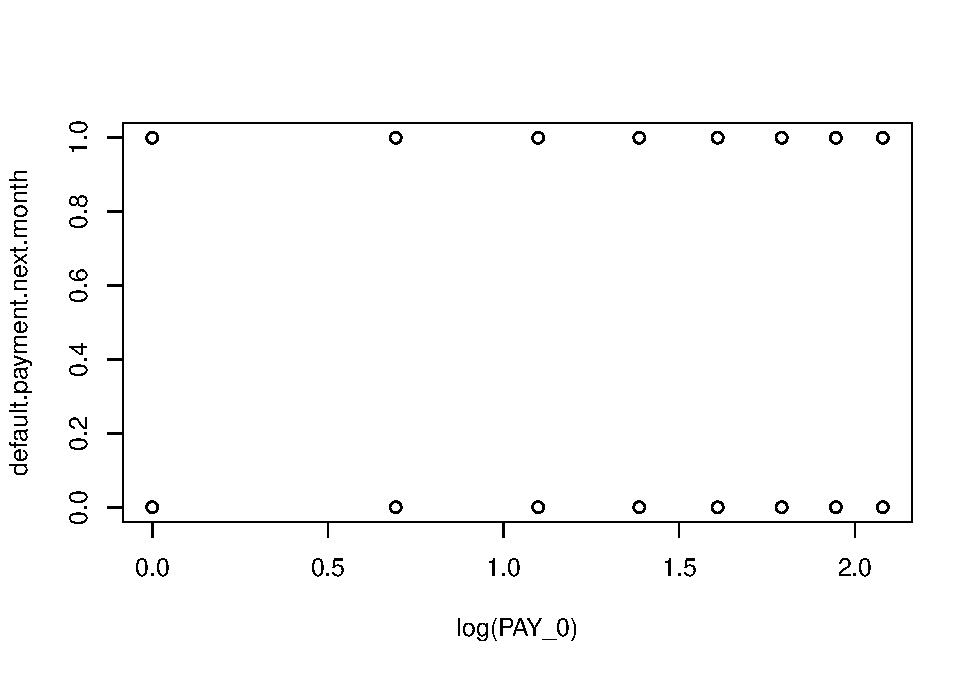
\includegraphics{Assignment-Q2_files/figure-latex/unnamed-chunk-10-6.pdf}

\begin{Shaded}
\begin{Highlighting}[]
\FunctionTok{print}\NormalTok{(qstats\_bct)}
\end{Highlighting}
\end{Shaded}

\begin{verbatim}
##                            Z1          Z2         Z3         Z4 AgostinoK2    N
##    0.5 to  100.5   0.34039810 -0.18954334 -0.7693713 -1.3338831  2.3711762  100
##  100.5 to  200.5   0.66913762  2.19838902  0.2247266 -0.7676373  0.6397690  100
##  200.5 to  300.5  -0.05333995 -0.90949858  1.3819421  1.4135294  3.9078292  100
##  300.5 to  400.5  -0.46149333 -1.79612967 -0.4851091 -0.6222045  0.6224693  100
##  400.5 to  500.5  -0.28138230 -2.32042975  1.2511699  0.6524407  1.9911049  100
##  500.5 to  600.5   0.39257006 -0.09466283  0.8627460 -0.6436196  1.1585769  100
##  600.5 to  700.5   1.34385978 -0.23854875  0.4574306  0.5028603  0.4621113  100
##  700.5 to  800.5  -1.62263124  1.24859798 -1.0873696 -0.2226075  1.2319269  100
##  800.5 to  900.5   1.11216769  0.83307642 -1.2887691  0.3480581  1.7820701  100
##  900.5 to 1000.5  -1.50882612  0.31832484  0.2683587  0.2379793  0.1286505  100
## TOTAL Q stats      8.96508902 16.72671515  8.2218433  6.0738410 14.2956843 1000
## df for Q stats     5.24317640  7.76626602  7.9998817  7.9999611 15.9998428    0
## p-val for Q stats  0.12480421  0.02933664  0.4120936  0.6389568  0.5766850    0
\end{verbatim}

\hypertarget{j-choose-between-the-models-and-give-a-reason-for-your-choice.}{%
\subsubsection{(j) Choose between the models and give a reason for your
choice.}\label{j-choose-between-the-models-and-give-a-reason-for-your-choice.}}

\end{document}
